\section{System Implementation}\label{implementation}
Fig.~\ref{fig2} shows the overall architecture of the NLP engine integrated into a docker infrastructure that includes three parts. The input files include the RA text file as well as the GSMA standard templates. The processing layer includes the logic associated with the NLP engine, i.e., the implementation of the designed methodology. The output file constitutes a JSON file populated with the classification of sub-articles as \textit{standard clauses}, \textit{customized texts} and \textit{variations}. In addition, each article includes the set of \textit{variables} it contains and each sub-article contains the specific \textit{variable} detected as long as it has been classified as \textit{variation} or \textit{customized texts}.

\begin{figure}[htbp]
\centerline{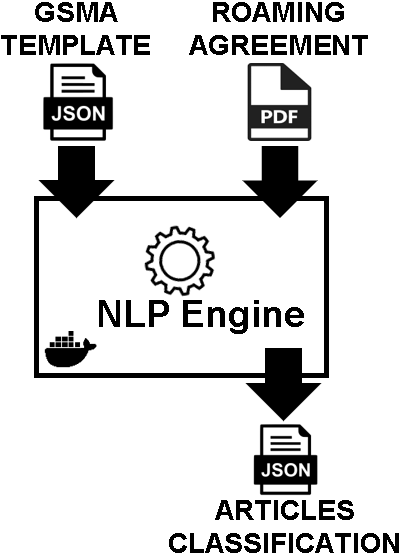
\includegraphics[width=0.20\textwidth]{images/NLP_Engine.png}}
\caption{NLP Engine overall architecture.}
\label{fig2}
\end{figure}

The input and output files are accessed by the container through Docker volumes. In addition, the NLP Engine has been developed as a Python v3.8 based library and therefore must be imported and run from an entry point. Although the NLP Engine constitutes a library, it must in turn, integrate other libraries such as boto3 (\cite{boto3}) and PyMuPDF (\cite{PyMuPDF}). Boto3 is a Software Development Kit (SDK) for Python, created and supported by Amazon Web Services (AWS). The NLP Engine imports the specific service associated with Amazon Comprehend. PyMuPDF constitutes another library imported into the NLP Engine to be used for headers and footers detection. Therefore, the docker image built for the NLP Engine must not only install the NLP Engine library but must also install the libraries it imports. The \textit{similarity} has been implemented in a pluggable way, therefore at code level, it is easy to change the \textit{Jaccard's similarity} for another one, e.g., cosine similarity \cite{Gupta2018}.

%\textcolor{red}{add link to github repo containing the full python code at some point?}